
\documentclass{standalone}

%Circular plate with distributed load
\usepackage{tikz}
\usepackage{pgfplots}
%\usepgfplotslibrary{patchplots}
%\pgfplotsset{compat=1.14}


\def\mystruct{\vphantom{hg}}

\pgfplotsset{
	legend image with text/.style={
		legend image code/.code={
		\node[anchor = center] at (0.3cm,0cm) {#1};
		}
	},width=12.8cm,height=9cm,compat=1.16,
}


\begin{document}



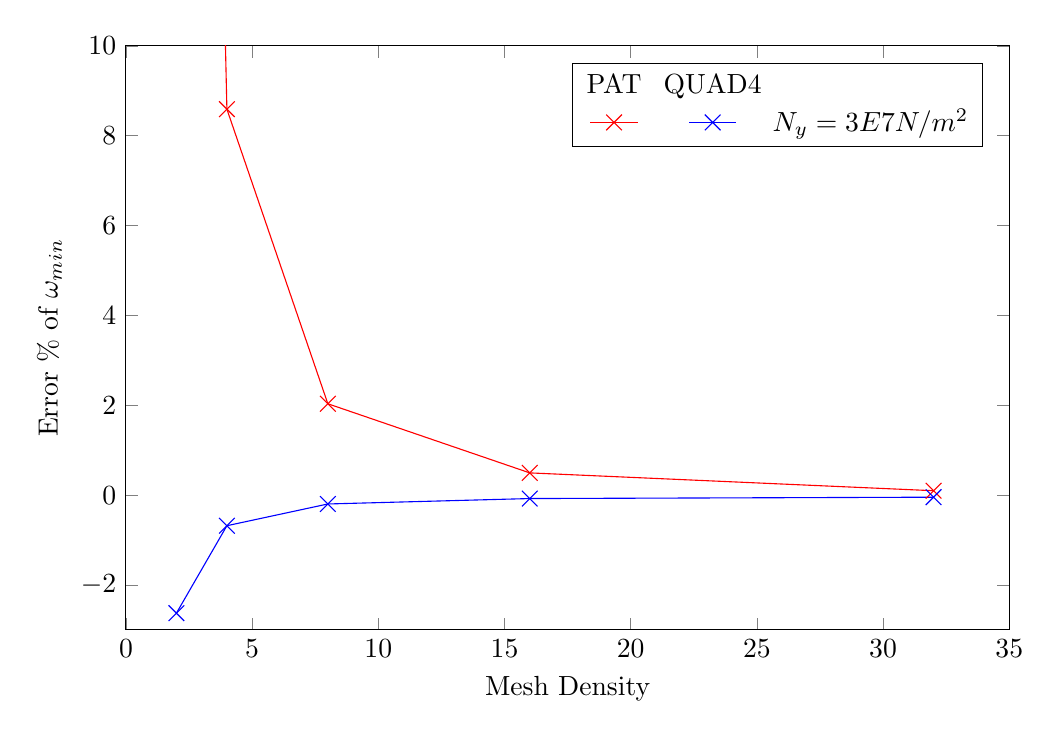
\begin{tikzpicture}
\begin{axis}[
%title={bla bla},
xlabel={Mesh Density},
ylabel={Error \% of $\omega_{min}$},
name=boundary,
legend columns = 2,
legend style = {
		legend cell align = left,
		},
	legend pos = north east,
		xmin=0,xmax=35,ymin=-3,ymax=10
]

\addlegendimage{legend image with text = PAT}
\addlegendentry{}

\addlegendimage{legend image with text = QUAD4}
\addlegendentry{}

%S_N_Tri
\addplot 
[red,
mark=x,mark options = {scale = 2,solid},
]
coordinates {(2,5.79795e+01)
(4,8.58982e+00)
(8,2.03382e+00)
(16,4.95137e-01)
(32,9.83703e-02)


};  \label{pgfplots:S_N_Tri}
\addlegendentry{}



%S_N_Rec
\addplot 
[blue,
mark=x,mark options = {scale = 2,solid},
]
coordinates {(2,-2.62648e+00)
(4,-6.80567e-01)
(8,-1.96694e-01)
(16,-7.59335e-02)
(32,-4.57567e-02)


}; \label{pgfplots:S_N_Rec}
\addlegendentry{$N_y=3E7 N/m^2$}












%\addplot 
%[
%solid,mark options = {scale = 2,solid},
%]
%coordinates {(0,0)
%(32,0)
%};


\end{axis}

%\node [draw,fill=white,inner sep=0pt,above left = %0.5em ] at (boundary.south east) {\small
%\begin{tabular} {cc}
%fel & zdf \\
%\ref{pgfplots:C_SS_P_Tri} & %\ref{pgfplots:C_SS_P_Rec} \\
%\end{tabular}

%};


\end{tikzpicture}


\end{document}